\chapter{Riemann--Roch Theorem}\label{ch:riemann-roch}
\begin{chout}
	With the conditions for inversion of the Laplacian behind us, we now prove the
	famous Riemann--Roch theorem.
\end{chout}

\section{Divisors}
In order to state the Riemann--Roch theorem, we first introduce the notion of a
divisor\sidenote{\footnotesize\cite[p. 129]{miranda}}. While initially an
abstract construction, divisors will allow us to jointly consider the zeros and
poles of a meromorphic function.

\begin{definition}[Divisor]
	A \defined{divisor} on a Riemann surface $ X $ is a function $ D:X \to
		\mathbb{Z} $ which has discrete support in $ X $.
\end{definition}

With the introduction of a formal summation notation, the idea of a divisor
become clearer. In particular, it is common to denote a divisor $ D $ by
\begin{align*}
	D=\sum_{p \in X}^{}{D(p) \cdot p},
\end{align*}
where $ D(p) \neq 0 $ only on a discrete subset of $ X $.

\begin{remark}
	We make an initial remark that in the same way as the discreteness of zeroes of
	meromorphic functions on all Riemann surfaces determined the finiteness of
	zeroes on \textit{compact} Riemann surfaces, the support of a divisor on a
	compact Riemann surface is necessarily finite.
\end{remark}

This remark is important, since it allows us to remove the formality of the sum
in construction of the following.

\begin{definition}[Degree]
	Let $ D $ be a divisor on a compact Riemann surface. The \defined{degree} of
	$ D $ is the sum of its values,
	\begin{align*}
		\deg(D) = \sum_{p \in X}^{}{D(p)}.
	\end{align*}
\end{definition}

There will be two particularly important examples of divisors for our
progression towards the Riemann--Roch theorem; those related to meromorphic
functions and $ 1 $-forms.

\begin{definition}[Principal divisor]
	A divisor is said to be \defined{principal} if it can be associated to the
	order of a meromorphic function,
	\begin{align*}
		(f) = \sum_{p \in X}^{}{\ord(f;p)\cdot p}.
	\end{align*}
\end{definition}

\begin{example}
	We have completely classified the meromorphic functions on the Riemann sphere
	as the rational functions, and aim to determine a general form for the
	principal divisor associated to these functions. Let
	\begin{align*}
		f(z) = c \cdot
		\frac{\prod_{i=1}^{n}{(z-z_i)^{e_i}}}{\prod_{j=1}^{m}{(z-z_j)^{f_j}}}
	\end{align*}
	be a general rational function on $ \hat{\mathbb{C}} $. Then,
	\begin{align*}
		\left( f \right) = \sum_{i=1}^{n}{e_i \cdot z_i} - \left(
		\sum_{j=1}^{m}{f_j} \right)\cdot \infty,
	\end{align*}
	since the function has zeroes of order $ e_i $ at the points $ \left\{ z_i
		\right\} $ and poles of order $ f_j $ at the points $ \left\{ z_j \right\} $.
\end{example}

\begin{definition}[Canonical divisor]
	A divisor is said to be \defined{canonical} if it can be associated to the
	order of a meromorphic $ 1 $-form,
	\begin{align*}
		(\omega) = \sum_{p \in X}^{}{\ord(\omega;p)\cdot p}.
	\end{align*}
\end{definition}

\begin{remark}
	It is common to denote the set of all divisors on a Riemann surface $ X $ by
	$ \mathrm{Div}(X) $, and this is in fact a group under pointwise addition.
	Furthermore, it follows directly from the definition that for $ f,g \in
		\mathcal{M}(X)\setminus \left\{ 0 \right\} $,
	\begin{gather*}
		(f g) = (f) + (g), \\
		(f/g) = (f) - (g), \\
		(1/f) = -(f),
	\end{gather*}
	and in particular, the principal divisors form a subgroup of $ \mathrm{Div}(X)
	$.
\end{remark}

It is logical now to make an attempt to organise the divisors, and in this vein,
we introduce a partial ordering. In particular, $ D \geq 0 $ if $ D(p) \geq 0
$ for all $ p $, and $ D \geq D' $ if $ D - D' \geq 0 $. From this partial
ordering, we can define\sidenote{\footnotesize\cite[p. 146]{miranda}} some
notable spaces of divisors.

\begin{definition}
	The space of meromorphic functions which have poles bounded by the divisor $ D
	$ is denoted and defined as,
	\begin{align*}
		L(D) = \left\{ f \in \mathcal{M}(X): (f) + D \geq 0 \right\}.
	\end{align*}
\end{definition}

Understanding of this space is most easily obtained by considering a single
point $ x \in X $. Suppose the divisor $ D $ is such that $ D(x) = n > 0 $.
Then, the condition that $ f \in L(D) $, is that $ (f) + D \geq 0 $ at $ x $,
which is in turn that $ \ord(f;x) + n \geq 0 $, i.e., the function $ f $ can
have a pole of at \textit{most} order $ n $ at the point $ x $.

Now consider the alternative, that $ D(x) = -n < 0 $. Then, with the same
logic as previously, $ \ord(f;x) - n \geq 0 $, and in particular, $ f $ must
have a zero of at \textit{least} order $ n $ at the point $ x $.

\begin{remark}
	If we take $ D $ to be the trivial divisor, then the space of meromorphic
	functions bounded by this divisor is exactly the space of holomorphic
	functions. That is,
	\begin{align*}
		L(0) = \mathcal{O}(X)
	\end{align*}
	which is the space of constant functions for any compact $ X $.
\end{remark}

We could choose to define an analogous space for the meromorphic $ 1 $-forms,
although this would be unnecessary. Recall that by Lemma~\ref{lem:mero-1-forms},
two non-zero $ 1 $-forms are multiplicatively related by a unique meromorphic
function. Therefore, for a canonical divisor $ K= (\omega) $, the space
\begin{align*}
	L(K-D) & = \left\{ f \in \mathcal{M}(X): (f) + K - D \geq 0 \right\}        \\
	       & = \left\{ f \in \mathcal{M}(X): (f) + (\omega) - D \geq 0 \right\} \\
	       & = \left\{ f \in \mathcal{M}(X): (f \omega) - D \geq 0 \right\}     \\
	       & = \{ f \omega \in \mathcal{M}^{1}(X): (f \omega) - D \geq 0 \}
\end{align*}
is exactly the analogous construction we wanted.

\section{Cohomological precursors}
Historically, the Riemann--Roch theorem came to fruition in two
parts\sidenote{\footnotesize\cite[p. 192]{miranda}}. Riemann found a lower bound
for the dimension of $ L ( D ) $, and it was Riemann's student, Roch, who
provided the term needed for equality. We will approach our consideration of
this result in the same manner, but it is first necessary to prove some results
related to the cohomological concepts we introduced in
Chapter~\ref{ch:differential-forms}.

\begin{lemma}
	The map
	\begin{align*}
		i:\overline{\mathcal{O}^{1}}(X) \to H ^{0,1}(X):\omega \mapsto [ \omega ]
	\end{align*}
	is an isomorphism.
	\begin{proof}
		Firstly, we show that $ i $ is injective; in particular that $ \ker(i) $
		is trivial. To do this, consider an element $ [ \omega ]\in H ^{0,1}(X) $
		such that $ [ \omega ]=0 $. By the definition of the cokernel, this means
		that there exists some smooth function $ f \in \Omega^0(X) $ such that
		\begin{align*}
			\overline{\partial }f          & = \omega,          \\
			\partial \overline{\partial }f & = \partial \omega.
		\end{align*}
		By Proposition~\ref{prop:anti-hol}, we know that $ \partial \omega=0 $, and
		in particular,
		\begin{align*}
			\Delta f = 0.
		\end{align*}
		By Theorem~\ref{thm:main-thm} this function $ f $ must be unique up to
		additive constant, and since $ \Delta 0 = 0 $, $ f $ must be constant. This
		determines that
		\begin{align*}
			0 = \overline{\partial }f = \omega,
		\end{align*}
		hence $ \ker(i) $ is trivial, and $ i $ is injective.

		Now, to show that $ i $ is surjective, consider an element $ [ \theta ]\in H
				^{0,1}(X) $. We need to find an element $ \omega \in
			\overline{\mathcal{O}^{1}}(X) $ such that $ i ( \omega ) = [ \theta ] $ that
		is, we need to find a smooth function $ \phi $ such that,
		\begin{align*}
			\omega = \theta + \overline{\partial }\phi.
		\end{align*}
		This is equivalent to,
		\begin{align*}
			\partial \omega & = \partial \theta + \partial \overline{\partial }\phi \\
			0               & = \partial \theta + \partial \overline{\partial }\phi \\
			\Delta \phi     & = 2i\partial \theta.
		\end{align*}
		Since
		\begin{align*}
			\int_{X}{\partial \theta} = \int_{X}{\d{\theta}} = \int_{\partial
				X}{\theta}=0,
		\end{align*}
		Theorem~\ref{thm:main-thm} determines the existence of $ \phi $.
	\end{proof}
\end{lemma}

\begin{remark}
	This provides some unification of our understanding. It was clear that $
		\mathcal{O}^{1}(X) \cong H ^{1,0}(X) $, and we know have that $
		\overline{\mathcal{O}^{1}}(X) \cong H ^{0,1}(X) $.
\end{remark}

\begin{lemma}
	The map
	\begin{align*}
		v: \mathcal{O}^{1}(X) \oplus \overline{\mathcal{O}^{1}}(X) \to H^1(X): (
		\omega_1, \omega_2 ) \mapsto [ \omega_1+\omega_2 ]
	\end{align*}
	is an isomorphism.
	\begin{proof}
		The proof uses a similar strategy to that employed for the previous lemma,
		and we choose not to spell out the details.
	\end{proof}
\end{lemma}

With these two lemmas, both of which are essentially consequences of
Theorem~\ref{thm:main-thm}, we obtain the following result.

\begin{theorem}[Hodge decomposition theorem]
	For a compact Riemann surface $ X $,
	\begin{align*}
		H^1(X) \cong H ^{1,0}(X) \oplus H ^{0,1}(X).
	\end{align*}
\end{theorem}

It can be shown\sidenote{\footnotesize\cite[p. 80]{griffiths}}, that the
dimension of the first de Rham cohomology group $ H^1(X) $ for a compact Riemann
surface $ X $ is equal to $ 2g $ where $ g $ is the genus. We are most
interested in the dimension of the Dolbeault cohomology groups, for reasons
which will soon become clear, and the following result quenches this interest.

\begin{lemma}
	For a compact Riemann surface $ X $, $ H ^{1,0}(X) \cong H ^{0,1}(X) $.
	\begin{proof}
		Recognising that the conjugation map,
		\begin{align*}
			\overline{\, \cdot\,}: \mathcal{O}^{1}(X) \to \overline{\mathcal{O}^{1}}(X):
			\omega \mapsto \overline{\omega}
		\end{align*}
		is an invertible, linear transformation and equivalently an isomorphism,
		gives,
		\begin{align*}
			H ^{1,0}(X) \cong \mathcal{O}^{1}(X) \cong \overline{\mathcal{O}^{1}}(X)
			\cong H ^{0,1}(X)
		\end{align*}
		as needed.
	\end{proof}
\end{lemma}

In particular, a basic linear algebraic argument allows us to state that the
dimension of both of $ H ^{1,0}(X) $ and $ H ^{0,1}(X) $ is $ g $ for a compact
Riemann surface of genus $ g $, i.e., half of the dimension of $ H^1(X) $.

\begin{corollary}\label{cor:dual-space-iso}
	For a compact Riemann surface $ X $, the dual space $ ( H^{0,1}(X) )^{*} $ is
	isomorphic to $ H^{1,0}(X) $.
	\begin{proof}
		Since vector spaces of the same finite dimension are isomorphic,
		\begin{align*}
			H^{1,0}(X)\cong H^{0,1}(X)\cong ( H^{0,1}(X) )^{*}.
		\end{align*}
	\end{proof}
\end{corollary}

\section{Riemann--Roch theorem}\label{sec:riemann-roch}
In the first part of this section, we aim to solve the problem of existence of
meromorphic functions. Given the results, we have obtained in the previous
section, it will be useful to rephrase our problem to relate to the Dolbeault
cohomological groups.

\begin{marginfigure}[-2\baselineskip]
	\centering
	\includegraphics{riemann-ineq/figure}
	\caption{Constructing the smooth cutoff function $ \beta $.}
\end{marginfigure}

\begin{lemma}\label{lem:riemann-existence}
	$ \hat{\mathbb{C}} $ admits a non-constant meromorphic function.
	\begin{proof}
		Let us consider a single point $ p \in \hat{\mathbb{C}} $. We aim to
		construct a meromorphic function on $ \hat{\mathbb{C}} $ which has a simple
		pole at $ p $. In order to do this, consider the chart domain $ U_p $
		containing $ p $, and let $ z $ be a local coordinate in this chart. In this
		chart domain, $ 1/z $ is a meromorphic function, and we can extend this
		globally by introducing a \defined{cutoff function} $ \beta $. We define $
			\beta $ such that $ \supp ( \beta )\subset U_p $, and equal to $ 1 $ near $
			p$.

		The product $ \beta/z $ can be regarded as a function over $ X $; extending
		by zero outside of $ U_p $. Hence, the problem of finding a meromorphic
		function with a simple pole at $ p $ is equivalent to finding a function $ g
			\in \Omega^0(X) $ such that $ g+\beta/z \in \mathcal{O}( X \setminus \{ p \}
			) $.

		By Proposition~\ref{prop:hol} we know that this is equivalent to,
		\begin{align*}
			\overline{\partial }\left( g + \beta \cdot \frac{1}{z} \right)=0 \iff
			\overline{\partial }g = - \overline{\partial }\left( \beta \cdot \frac{1}{z}
			\right).
		\end{align*}

		A further application of Proposition~\ref{prop:hol}, and relabelling $ A =
			\overline{\partial }( \beta )1/z $, gives the simplification,
		\begin{align*}
			\overline{\partial }g = -A.
		\end{align*}
		If we consider the corresponding class $ [ A ]\in H ^{0,1}(X) $, we can see
		that the existence of a smooth function $ g $, is equivalent to the
		condition that $ A \in \im ( \overline{\partial } ) $, which is in turn
		equivalent to $ [ A ] = [ 0 ]\in H ^{0,1}(X) $. Our work in the previous
		section allows us to state that $ \dim H ^{0,1}(X)=0 $, which is enough to
		guarantee the existence of the function $ g $.
	\end{proof}
\end{lemma}

This is the most basic case in the proof of the following theorem. While we will
not provide a proof, it is intuitively clear how to proceed given a Riemann
surface of higher genus; adding sufficiently many poles, or in particular
sufficiently increasing $ \deg(D) $, forces a linear dependence between the
elements of the $ H ^{0,1}(X) $, which allows for the construction of the
promised meromorphic function.

\begin{theorem}[Riemann--Roch inequality]
	For a compact Riemann surface $ X $ of genus $ g $, and a divisor $ D $,
	\begin{align*}
		\dim L(D) \geq \deg(D) + 1 - g.
	\end{align*}
\end{theorem}

\begin{corollary}
	Every compact Riemann surface has a non-constant meromorphic function.
	\begin{proof}
		This follows directly from Riemann's inequality. If we take $ \deg(D) >g $,
		then
		\begin{align*}
			\dim L(D) \geq \deg(D) + 1 - g > g + 1 - g = 1,
		\end{align*}
		and hence there must be a non-constant function in $ L(D) $.
	\end{proof}
\end{corollary}

\begin{corollary}
	If $ X $ is a compact Riemann surface of genus $ 0 $, then $ X \cong
		\hat{\mathbb{C}} $.
	\begin{proof}
		If we take $ \deg(D)=1 $,
		\begin{align*}
			\dim L(D) \geq \deg(D)+1-g = 2,
		\end{align*}
		and in particular, there exists a meromorphic function which has a single,
		simple pole. Let $ p $ be this point, let $ \varphi:X \to \mathbb{C} $ be
		this function, and $ \Phi:X \to \hat{\mathbb{C}} $ the corresponding
		holomorphic representation. Then $ \deg(\Phi) = \deg(\Phi;\infty) =
			\mult(\Phi;p)=1 $, and hence $ \Phi $ is bijective, and further to this, a
		biholomorphism.
	\end{proof}
\end{corollary}

As mentioned previously, it was Gustav Roch, a student of Riemann, who
strengthened the inequality to an equality by incorporating the space of
meromorphic $ 1 $-forms associated to a canonical divisor. We will prove the first
case of the theorem, that is in the case where $ D $ is a non-negative divisor,
following Donaldson\sidenote{\footnotesize\cite[p. 115]{donaldson}}. We need a
final definition to prove the theorem in this restricted form.

\begin{definition}[Tangent residue]
	Let $ p \in X $ for a compact Riemann surface $ X $. Let $ f $ have a local
	Laurent series expansion about the point $ p $ as,
	\begin{align*}
		f = \sum_{i=-1}^{\infty}{a_{i}z^{i}}
	\end{align*}
	where $ z $ is the local coordinate centred at $ p $. Then, the
	\defined{tangent residue} of $ f $ is $ a_{-1}\frac{\partial }{\partial z} \in
		TX_{p} $ where $ TX_{p} $ denotes the tangent space at $ p $.
\end{definition}

\begin{marginfigure}
	\centering
	\resizebox{\columnwidth}{!}{
		\includegraphics{tangent-space/figure}
	}
	\caption{A visualisation of $ T \hat{\mathbb{C}}_{p} $.}
\end{marginfigure}

\begin{theorem}[Riemann--Roch theorem]
	Let $ X $ be a compact Riemann surface, and $ K $ a canonical divisor on $ X $.
	Then, for any divisor $ D $,
	\begin{align*}
		\dim L(D) - \dim L(K-D) = \deg(D) + 1 - g.
	\end{align*}
	\begin{proof}
		As stated above, we will consider the case where $ D = p_{1}+ \cdots + p_{d}
		$ for $ p_{i} $ distinct points of $ X $. In this case, $ L(D) $ is the
		space of meromorphic functions which have at worst simple poles at each of
		the $ p_{i} $. Furthermore, the space $ L(K-D) $ can be recognised as the
		space of holomorphic $ 1 $-forms which vanish at each of the $ p_{i} $. This
		is understood by considering the fact that $ \omega \in L ( K-D ) \implies (
			\omega ) \geq D $, which imposes that $ \ord ( \omega;p_{i} ) \geq 1 $ for
		each $ 1 \leq i \leq d $.

		We aim to build the proof in stages, in an argument which relies heavily on
		results from linear algebra. Firstly, consider the inclusion defined as
		\begin{align*}
			I:\mathbb{C}\to L ( D ):c \mapsto f_{c} & : \mathbb{C}\to \mathbb{C} \\
			                                        & : z \mapsto c,
		\end{align*}
		i.e., a map which takes the constants in $ \mathbb{C} $ to their respective
		constant maps $ f_{c} $. We can make initial note of the fact that the image
		of $ I $, $ \im I $, is the set of complex valued constant functions.

		We consider also the map
		\begin{align*}
			R: L(D) \to \bigoplus_{i=1}^{d}{TX_{p_{i}}},
		\end{align*}
		which maps the meromorphic function $ f $ to its tangent residues in the
		local coordinates $ z_{i} $ of each of the $ p_{i} $. The kernel of the map,
		is the collection of functions which have zero residue at every one of the
		$ p_{i} $, and since we are considering the case of $ D(p) \in \{ 0,1 \} $,
		this is exactly the set of holomorphic functions. Furthermore, we know that
		holomorphic functions are constant, and therefore, $ \ker R = \im I $. In
		particular, we have an exact sequence of vector spaces,
		\begin{align*}
			\mathbb{C}\xrightarrow{\ I\ } L(D)\xrightarrow{\ R\ }
			\bigoplus_{i=1}^{d}{TX_{p_{i}}}.
		\end{align*}
		We can relate the dimensions of these spaces using the rank nullity theorem,
		\begin{align*}
			\dim L(D) & = \dim\im R + \dim\ker R \\
			          & = \dim\im R + \dim\ker I \\
			          & = \dim\im R + 1,
		\end{align*}
		hence our interest now lies in the space $ \im R $.

		In the same vein as our previous work, we aim to find a map whose kernel is
		the same as $ \im R $. With this in mind, we consider the family of maps
		\begin{align*}
			A_{i}:TX_{p_{i}} \to H^{0,1}(X),
		\end{align*}
		which for a local coordinate $ z_{i} $ centered on $ p_{i} $, maps $
			\partial/\partial z_{i} $ to the cohomology class $ [ A_{i} ] $ where $
			A_{i} $ is defined in the same way as in the proof of
		Lemma~\ref{lem:riemann-existence}, that is, as the global extension of $
			\overline{\partial}( \beta_{i} \cdot 1/z_{i} ) $. We therefore have a map
		\begin{align*}
			\underline{A}: \bigoplus_{i=1}^{d}{TX_{p_{i}}} \to H^{0,1}(X):
			( t_{1},...,t_{d} )\mapsto \sum_{i=1}^{d}{A_{i}( t_{i} )}.
		\end{align*}
		and aim to show that $ \im R = \ker \underline{A} $. To begin, consider
		an element $ R ( f ) = ( \lambda_{1}\cdot \partial/\partial z_{1},...,
			\lambda_{d}\cdot \partial/\partial z_{d} ) $, and the map
		\begin{align*}
			F = f - \sum_{i=1}^{d}{\lambda_{i}\beta_{i}\frac{1}{z_{i}}},
		\end{align*}
		which is, by design a smooth function on $ X $. Therefore, $ [
					\overline{\partial }F ]=0 $ in $ H^{0,1}(X) $, and furthermore, since $ f $
		is holomorphic away from the points $ p_{i} $, $ \overline{\partial }f=0 $
		away from these points, and a natural extension to $ 0 $ over these points
		gives,
		\begin{align*}
			\left[\overline{\partial }\left(
			\sum_{i=1}^{d}{\lambda_{i}\beta_{i}\frac{1}{z_{i}}} \right) \right] & =
			[\overline{\partial }f ]                                                   \\
			\left[\overline{\partial }\left(
			\sum_{i=1}^{d}{\lambda_{i}\beta_{i}\frac{1}{z_{i}}} \right) \right] & = 0  \\
			\sum_{i=1}^{d}{\lambda_{i}[ A_{i} ]}                                & = 0,
		\end{align*}
		and in particular, $ \im R \subseteq \ker \underline{A} $. To show the other
		inclusion, consider $ \underline{\alpha} = ( \alpha_{1}\partial/\partial
			z_{1},..., \alpha_{d}\partial/\partial z_{d} )\in \ker \underline{A} $. By
		the definition of $ \underline{A} $, this is equivalent to
		\begin{align*}
			\underline{A}( \underline{\alpha} ) = 0 \in H^{0,1}(X),
		\end{align*}
		which is equivalent to the existence of a function $ g \in \Omega^{0}(X) $
		such that,
		\begin{align*}
			\overline{\partial }g = - \underline{A}( \underline{\alpha} ).
		\end{align*}
		Rearranging this expression gives us that
		\begin{align*}
			\overline{\partial }\underbrace{\left( g+
				\alpha_{1}\beta_{1}\frac{1}{z_{1}}+ \cdots +
				\alpha_{d}\beta_{d}\frac{1}{z_{d}} \right)}_{G \in L(D)}=0,
		\end{align*}
		and since $ R(G)=\underline{\alpha} $, $ \ker \underline{A}\subseteq \im R
		$, and in particular $ \im R = \ker \underline{A} $.

		Hence we can extend our exact sequence,
		\begin{align*}
			\mathbb{C}\xrightarrow{\ I\ } L(D)\xrightarrow{\ R\ }
			\bigoplus_{i=1}^{d}{TX_{p_{i}}}\xrightarrow{\ \underline{A}\ } H^{0,1}(X),
		\end{align*}
		and rephrase our previous expression as,
		\begin{align*}
			\dim L(D) & = \dim\ker \underline{A} + 1.
		\end{align*}

		In order to compute $ \dim\ker \underline{A} $, we consider the transpose of
		this map,
		\begin{align*}
			\underline{A}^{T}: \left( H^{0,1}(X) \right)^{*}\to \left(
			\bigoplus_{i=1}^{d}{TX_{p_{i}}} \right)^{*} = \bigoplus_{i=1}^{d}{T
				^{*}X_{p_{i}}},
		\end{align*}
		and use elementary linear algebraic relations, together with the fact that $
			\dim H^{0,1}(X)=g $,
		\begin{align*}
			\dim\bigoplus{TX_{p_{i}}} - \dim H^{0,1}(X) & = \dim\im \underline{A} +
			\dim\ker \underline{A}
			\\ & \quad - \dim\im
			\underline{A}^{T} - \dim\ker
			\underline{A}^{T}
			\\ \deg(D)-g
			                                            & = \dim\ker \underline{A} -
			\dim\ker \underline{A}^{T}.
		\end{align*}

		From Corollary~\ref{cor:dual-space-iso} we know that $ ( H^{0,1}(X)
			)^{*}\cong H^{1,0}(X) $ and consequently, we define a final map
		\begin{align*}
			E:H^{1,0}\to \bigoplus_{i=1}^{d}{T ^{*}X_{p_{i}}}:\omega \mapsto (
			\omega ( p_{1} ),..., \omega ( p_{d} ) ).
		\end{align*}

		It can be shown\sidenotemark\ that $ \underline{A}^{T} = 2 \pi i E $, and
		noticing that $ \ker E$ is the space of holomorphic $ 1 $-forms which vanish
		at every point $ p_{i} $ gives,
		\begin{align*}
			\dim L(D)                              & = 1 + \dim\ker \underline{A} \\
			\dim L(D) - \dim\ker \underline{A}^{T} & = 1 + \deg(D) - g            \\
			\dim L(D) - \dim\ker E                 & = 1 + \deg(D) - g            \\
			\dim L(D) - \dim L(K-D)                & = 1 + \deg(D) - g.
		\end{align*}
	\end{proof}
\end{theorem}
\sidenotetext[][-10\baselineskip]{\footnotesize\cite[p. 116]{donaldson}}
